%===================================== CHAP 5 =================================

\chapter{Analysis}

Figure \ref{fig:epsilon_big_range} shows the effect of the privacy parameter $\epsilon$.

\begin{figure}[h!]
	\centering
	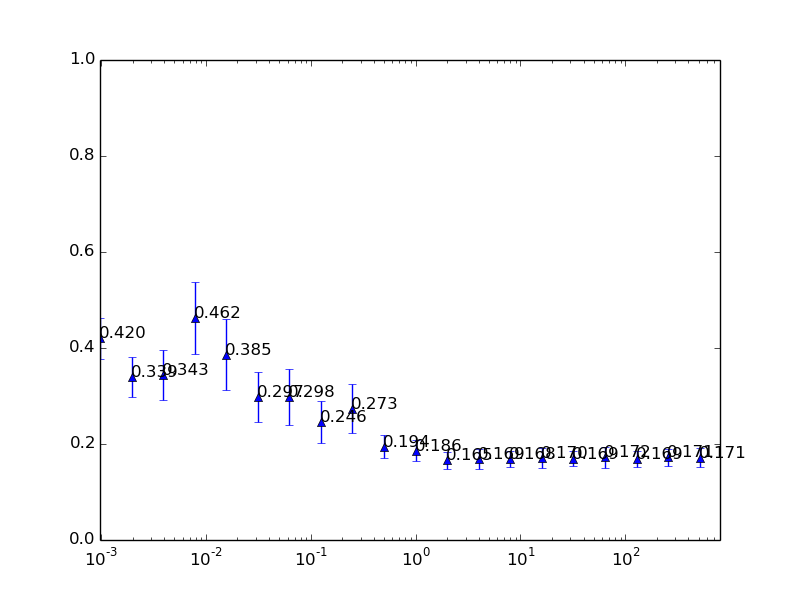
\includegraphics[width=\textwidth]{fig/eps2e-10-2e9,bud=eps,peers50,groups50,reg2e-4}
 	\caption{$\epsilon = [2^{-10}, 2^{9}], \lambda = 2^{-4}$, 50 peers, 1 aggregation}
 	\label{fig:epsilon_big_range}
\end{figure}
 

 
\begin{figure}[h!]
	\centering
	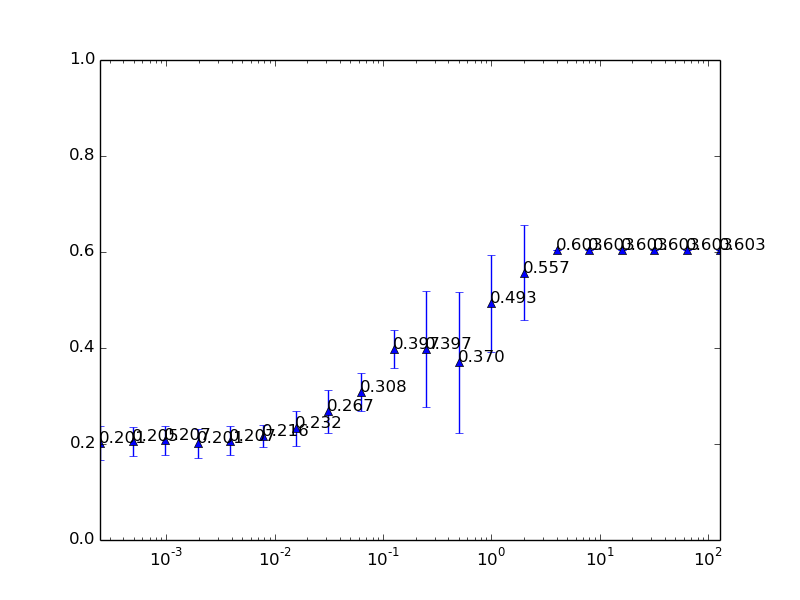
\includegraphics[width=\textwidth]{fig/eps2e10.0,bud2e10.0,peers10,groups5,reg2e-12-2e7}
	\caption{$\epsilon = 2^{10}, \lambda = [2^{-12}, 2^{7}]$, 50 peers, 1 aggregation}
	\label{fig:regularization_extremelyhighepsilon}
\end{figure}

Figure \ref{fig:regularization_extremelyhighepsilon} shows the normal effect regularization has on accuracy. As the regularization parameter $\lambda$ grows large, the model becomes less able to fit the training data, eventually resulting in models predicting only the negative class. On this particular dataset it appears that a logistic regression model is not at risk of overfitting, since the cross validated error does not increase when the level of regularization is very low. In a context where privacy is irrelevant, this would mean that selecting some regularization parameter in the range $[10^{-5},10^{-2}]$ could be acceptable. Choosing a level at the high end of this range could be a good idea, to reduce risk of overfitting.

When noise, tuned to offer $epsilon$-differential privacy, is added to the model creation process, the trade-offs involved in choosing regularization $\lambda$ become more tricky.

What are the results of our experiments?

What did we learn from the basic structure of creating our framework?

What difficulties did we encounter?

What can we take away from our experiments?

What should have been done better? 

What did we learn from tuning the different parameters?

More data per peer leads to better classification. With small number of peers, there are more records per peer. This generally leads to better classification accuracy. Why is this? 

Australian: Sweet spot for regularization at a 2e-3, 10 peers 5 groupsize

What was the effect of tuning the regularization parameter? High and low regularization leads to more SD on the error rate, but there is a sweet spot.

What was the effect of increasing the epsilon? 
	It seemed like it was better to keep the perUpdateBudget smaller than the epsilon, so that the models are aggregated more. Did this lead to better accuracy? Why do more aggregations lead to better classification than having a bigger budget but only one aggregation.
	
Compare the results of our distributed logistic regression classifier with the tradional ones in literature. Sharma and Arora \cite{sharma2013adaptive} report getting 92.95\% classification accuracy on the same data set. Kumar et al\cite{kumar2012comparative}. reports  0.1389 error rate before filtering when using logistic regression combined with a least squares regularization method. Our classifier can compare to these under certain circumstances, even after noise addition.  


\cleardoublepage